\documentclass[main.tex]{subfiles}

\begin{document}

\section{服务端系统设计}

虽然本课程的主要教学重点是移动互联网技术和移动互联网应用开发的,但是对于一个在线多媒体播放系统而言,如果没有服务端的设计和实现,移动端的应用程序只会是无根之木和无水之萍。因此在本节中,我们将就服务端实现中的总体架构和重点逻辑进行阐述,供参考。

\subsection{服务端总体架构}

本系统的服务端使用ASP.NET Core进行开发,在开发的过程中使用典型的MVC架构进行开发,系统的架构如图\ref{fig:server-architecture}所示。

\begin{figure}[htbp]
    \centering
    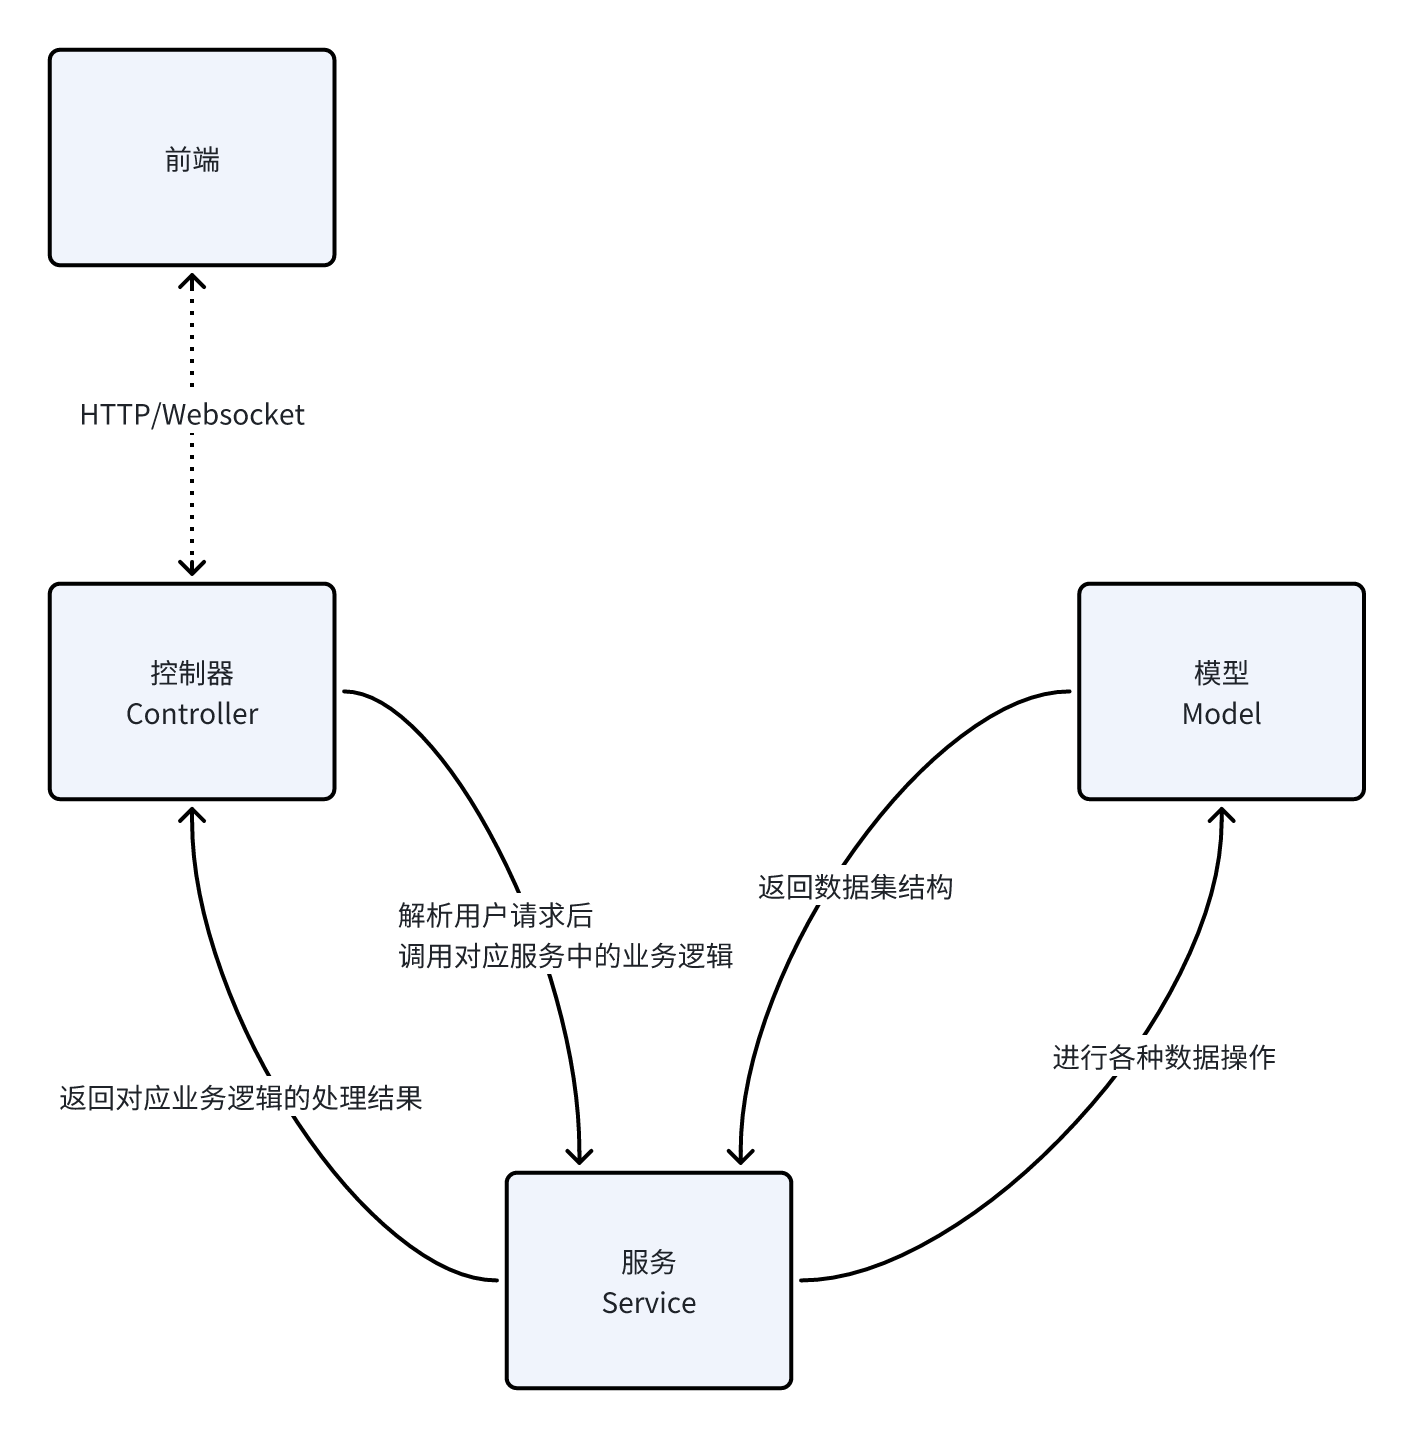
\includegraphics[width=0.8\textwidth]{assets/server-architecture.png}
    \caption{服务端架构图}
    \label{fig:server-architecture}
\end{figure}

在系统的架构中主要有如下几个部分组成:
\begin{itemize}
    \item 模型层,是系统架构中的底层,也就是系统中的数据存取层。在这一层主要负责系统中需要和数据库进行交互的部分逻辑。
    \item 服务层,是系统架构中的中层,是系统中业务逻辑主要存在的层。在这一层中负责完成系统需要完成的各种复杂逻辑,对下同模型层进行交互完成数据的增、删、查、改。对上同控制器层进行交互处理用户的请求。
    \item 控制器层,是系统架构中的顶层,直接定义了同前端进行交互的逻辑。在这一层中声明了向前端提供各种接口的地址、请求方式和请求体,并负责对前端发送的请求进行校验和序列化为对象,在调度对应的服务得到结果之后序列化发送给前端。
\end{itemize}

\subsection{多媒体文件的扫描和元数据的获取}

在服务端中的核心逻辑之一便是如何快速而高效的从用户指定的媒体文件夹下扫描多媒体文件并从中提取出多媒体文件的元数据。本节中便重点阐述本段逻辑。

\begin{lstlisting}[style=csharp]
    private async Task<IEnumerable<Song>> ScanSongAsync(DirectoryInfo directory, CancellationToken cancellationToken)
    {
        ConcurrentBag<Song> songs = [];

        await Parallel.ForEachAsync(directory.EnumerateDirectories(), cancellationToken, async (info, token) =>
        {
            foreach (Song song in await ScanSongAsync(info, token))
            {
                songs.Add(song);
            }
        });

        await Parallel.ForEachAsync(directory.EnumerateFiles(), cancellationToken, async (f, _) =>
        {
            if (!MediaItemTypes.MusicTypes.Contains(f.Extension))
            {
                return;
            }

            try
            {
                TagLib.File tagFile = TagLib.File.Create(f.FullName);

                IPicture? picture = tagFile.Tag.Pictures.FirstOrDefault();
                string? coverImageUrl = null;
                if (picture is not null)
                {
                    coverImageUrl = "/api/file/" + await fileStore.UploadFileAsync(picture.Data.Data, picture.MimeType);
                }

                Song song = new()
                {
                    Title = tagFile.Tag.Title ?? f.Name,
                    Arist = tagFile.Tag.FirstPerformer ?? "Default Arist",
                    Path = f.FullName,
                    Url = $"/api/file/{await fileStore.ClarifyLocalFileAsync(f.FullName, tagFile.MimeType)}",
                    CoverImageUrl = coverImageUrl ?? string.Empty,
                    Album = new Album
                    {
                        // 避免空应用错误
                        Title = tagFile.Tag.Album ?? "Default Album",
                        Arist = tagFile.Tag.FirstAlbumArtist ?? "Default Artist",
                        Path = f.Directory is null ? string.Empty : f.Directory.FullName,
                        ParentRepository = new MediaRepository()
                    }
                };

                songs.Add(song);
            }
            catch (UnsupportedFormatException e)
            {
                logger.LogInformation("Failed to parser file {}: {}.", f.Name, e);
            }
        });

        return songs;
    }
\end{lstlisting}

这段代码是用于扫描指定目录及其子目录下所有音乐文件,并从中提取元数据以创建Song对象的异步方法。这个方法不仅读取音乐文件的元数据(如标题、艺术家、专辑等),还尝试从文件中获取封面图片并上传到一个文件存储服务。

该递归方法接收一个DirectoryInfo对象和一个CancellationToken作为参数,用于取消正在进行的任务。使用ConcurrentBag<Song>来收集所有找到的歌曲信息。ConcurrentBag是线程安全的集合类型,适合多线程操作。Parallel.ForEachAsync用于异步并行地遍历目录下的所有子目录,递归调用ScanSongAsync方法。这样可以有效地利用多核处理器进行并行处理。

方法的核心是文件过滤和元数据提取。方法对目录下的所有文件进行遍历,仅处理扩展名属于预定义的MediaItemTypes.MusicTypes集合的文件。使用TagLib库读取音频文件的元数据,如标题、艺术家、专辑信息等,并尝试从音频文件中提取封面图片,并将其上传到文件存储服务,通过调用fileStore.UploadFileAsync方法。上传成功后,封面图片的URL被保存在Song对象中。如果遇到不支持的文件格式,会捕获UnsupportedFormatException异常,并记录相关信息。这有助于调试和避免因个别文件问题导致整个扫描过程失败。最终,该方法返回一个IEnumerable<Song>集合,包含了所有扫描到的歌曲信息。

\subsection{实时转码和推流实现}

服务端中的核心代码是实现视频的实时转码和推流,这是在服务端通过调用FFmpeg程序来实现的。

\begin{lstlisting}[style=csharp]
public record VideoConversion(Task<IConversionResult> RunningTask,
    DirectoryInfo CacheDirectory,
    string Name,
    CancellationTokenSource CancellationTokenSource);

public class FfmpegService
{
    public VideoConversion? CurrentConversion { get; set; }

    public async Task<IConversionResult> StartConversion(FileInfo video, DirectoryInfo cacheDirectory, string name,
        CancellationToken cancellationToken)
    {
        IMediaInfo inputVideo = await FFmpeg.GetMediaInfo(video.FullName, cancellationToken);

        IConversion conversion = FFmpeg.Conversions.New()
            .AddStream(inputVideo.Streams)
            .AddParameter("-re", ParameterPosition.PreInput)
            .AddParameter("-c:v h264 -f hls")
            .AddParameter("-profile:v high10")
            .AddParameter("-hls_list_size 10 -hls_time 10 -hls_base_url /api/hls/")
            .AddParameter("-hls_flags delete_segments")
            .SetOutput(Path.Combine(cacheDirectory.FullName, $"{name}.m3u8"));

        return await conversion.Start(cancellationToken);
    }
}
\end{lstlisting}

这段C\#代码定义了一个FfmpegService类,用于处理视频转换任务,特别是将输入视频文件转换为HLS流格式,以便于在网络环境中播放。

VideoConversion是一个记录类型,它封装了一个正在进行的视频转换任务的状态。包括正在运行的任务(Task<IConversionResult>)、缓存目录(DirectoryInfo)、转换任务的名称(string)以及用于取消任务的CancellationTokenSource。这种设计允许外部代码追踪当前正在进行的转换任务状态,同时提供了一种优雅地取消转换任务的方法。

FfmpegService类中有一个CurrentConversion属性,它是VideoConversion?类型(可空的VideoConversion)。这意味着FfmpegService实例可以跟踪当前正在执行的视频转换任务。

StartConversion方法接受一个视频文件(FileInfo)、缓存目录(DirectoryInfo)、任务名称(string)和取消令牌(CancellationToken)作为参数。首先,它使用FFmpeg库的GetMediaInfo方法异步获取输入视频的媒体信息。然后,它创建一个新的转换流程,添加视频流信息、设置编码参数和输出格式。这里特别配置了HLS流的参数,例如-c:v h264表示使用H.264编码,-profile:v high10指定了编码的配置文件,-hls\_list\_size和-hls\_time控制了HLS播放列表的大小和片段持续时间。最后,它设置了输出文件路径(.m3u8格式的HLS播放列表)并启动转换任务,返回IConversionResult类型的异步任务。

该方法的设计提高了视频处理的效率,还提供了灵活的取消机制,这对于长时间运行的任务尤其重要。


\end{document}